\documentclass[12pt]{article}

\usepackage{lmodern}
\usepackage[T1]{fontenc}
\usepackage[spanish,activeacute]{babel}
\usepackage[utf8]{inputenc}
\usepackage{mathtools}
\usepackage{enumerate}
\usepackage{amsthm}
\usepackage{amssymb}
\usepackage[hidelinks]{hyperref}
\usepackage{anysize}
\usepackage{listings}
\usepackage{float}
\usepackage{hyperref}
\usepackage{graphicx}

\marginsize{2cm}{2cm}{2cm}{2cm}

\lstset{ %
escapeinside=||,
language=python,
basicstyle=\small}

\title{Metaheur\'isticas:\\
 Pr\'actica 3.b: Algoritmos Genéticos para el Problema de Selección de Características.}
\author{Anabel G\'omez R\'ios.\\
 DNI: 75929914Z.\\
 E-mail: anabelgrios@correo.ugr.es}


\begin{document}
\maketitle

\begin{center}
Curso 2015-2016\\

Problema de Selección de Características.\\ 

Grupo de prácticas: Viernes 17:30-19:30\\

Quinto curso del Doble Grado en Ingeniería Informática y Matemáticas.\\
\textit{ }\\
\end{center}

Algoritmos considerados:
\begin{enumerate}
\item Algoritmo Genético Generacional.
\item Algoritmo Genético Estacionario.
\end{enumerate}

\newpage

\tableofcontents

\newpage

\section{Descripción del problema}
Queremos obtener un sistema que permita clasificar un conjunto de objetos en unas determinadas clases que conocemos previamente. Para ello disponemos de una muestra de dichos objetos ya clasificados y una serie de características para cada objeto.\\

El problema es, por tanto, construir un clasificador que se comporte lo suficientemente bien fuera de la muestra de la que disponemos, es decir, que clasifique bien nuevos datos. Para hacer esto, lo que hacemos es particionar la muestra en dos subconjuntos, uno que utilizaremos de entrenamiento para que el clasificador aprenda y otro que utilizaremos para test, es decir, para ver cómo de bien se comporta el clasificador que hemos obtenido con el primer subconjunto fuera de los datos de entrenamiento. Además haremos distintas particiones, en concreto 5, y construiremos un clasificador para cada una de ellas. Las particiones serán además proporcionadas (habrá el mismo número de muestras de una clase en el conjunto de entrenamiento y en el de test). Podemos comprobar cómo de bien se comporta cada clasificador porque sabemos en realidad las clases de los objetos que tenemos en la muestra y podemos comparar las verdaderas clases con las que el clasificador obtiene suponiendo que no dispusiéramos de ellas.\\
Buscamos pues en todo momento optimizar la tasa de acierto del clasificador.\\
Vamos a utilizar además validación cruzada: es decir, para cada partición en dos subconjuntos primero uno será el de entrenamiento y el otro el de test y después les daremos la vuelta y volveremos a construir un clasificador. La calidad por tanto de cada algoritmo será la media de los porcentajes de clasificación (la tasa de acierto) para estas 10 particiones.\\

Nos queda describir cómo aprende el clasificador con los datos de entrenamiento. Ya que podemos llegar a tener muchas características de las cuales algunas podrían ser poco o nada significantes, lo que hacemos es elegir un subconjunto de características que describan bien los datos de entrenamiento, de forma que en los datos de test sólo tenemos en cuenta este subconjunto de características a la hora de deducir cuál es la clase de cada nuevo dato. Para esta "deducción" vamos a utilizar la técnica de los 3 vecinos más cercanos (3-NN): buscamos para cada dato los tres vecinos más cercanos en el conjunto de entrenamiento (si el mismo dato al que le vamos a calcular la clase pertenece al conjunto de entrenamiento tenemos que sacarlo previamente del conjunto de entrenamiento. Esto es lo que se llama \textit{leave one out}) teniendo en cuenta las características seleccionadas hasta el momento, consultamos las clases de estos tres vecinos, nos quedamos con la clase que más veces aparezca (o, en caso de empate, con la clase del vecino más cercano) y ésta será la clase del dato. Para obtener la tasa de acierto lo que hacemos es repetir esto para todos los datos, comparar estas clases con las reales y contar el número de veces que acierta.\\

El cómo exploramos el espacio de búsqueda hasta encontrar la mejor solución (el subconjunto de características que da mayor tasa de acierto) es en lo que se diferencian los distintos algoritmos que vamos a ver en esta práctica.

\newpage

\section{Descripción de la aplicación de los algoritmos empleados al problema}
El primer paso común a todos los algoritmos es normalizar los datos de los que disponemos por columnas (es decir, por características) de forma que todas se queden entre 0 y 1 y no haya así preferencias de unas sobre otras.\\

A continuación se genera una población inicial, consistente en 30 cromosomas generados de forma aleatoria. Después, en cada iteración de los algoritmos, se irá seleccionando una parte de la población se cruzarán parte o todos de esta selección según una cierta probabilidad que ya comentaremos en cada caso. Una vez tenemos la nueva población se realizarán mutaciones según otra probabilidad y una vez termine todo el algoritmo nos quedaremos con la mejor solución obtenida en todos los casos, que será aquel cromosoma con la mayor tasa.\\

Los dos algoritmos tienen una condición de parada común, que es llamar a la función de evaluación 15000 veces.

\subsection{Esquema de representación de soluciones}
La representación elegida para las soluciones ha sido la binaria: un vector de $N$ posiciones, donde $N$ es el número de características, en el que aparece \textit{True} o \textit{False} en la posición $i$ según si la característica $i$-ésima ha sido seleccionada o no, respectivamente. Esta representación es la más sencilla y cómoda cuando no hay restricciones sobre el número de características a elegir, es decir, el número de características que se han de elegir lo aprende cada algoritmo, como es el caso de los algoritmos que vamos a utilizar.

\subsection{3-NN}
Como hemos comentado, la técnica para clasificar que vamos a utilizar en todos los algoritmos será el 3NN. Consiste en considerar, para cada dato, la distancia euclídea entre el dato y todos los demás, es decir, entre las características de los datos (excluyéndose él mismo en caso de que estuviéramos preguntando por algún dato dentro del conjunto de entrenamiento) y quedarnos con las clases de los 3 con la distancia más pequeña. La clase del dato en cuestión será de estas tres la que más se repita o, en caso de empate, la clase que corresponda al vecino más cercano.\\
En cada momento la distancia euclídea se calcula teniendo en cuenta las características que están seleccionadas en el momento, por lo que no podemos tener una matriz fija de distancias, hay que ir calculándolas sobre la marcha.

\subsection{Función de evaluación}
La función de evaluación será el rendimiento promedio de un clasificador 3-NN en el conjunto de entrenamiento: calcularemos la tasa para cada dato dentro del conjunto de entrenamiento haciendo el leave one out descrito anteriormente y nos quedaremos con la media de las tasas obtenidas. El objetivo será por tanto maximizar esta función.
La tasa se calcula como 100*(nº instancias bien clasificadas / nº total de instancias).\\

El pseudo-código es el siguiente:\\
\begin{lstlisting}
Obtener el subconjunto de entrenamiento que se va a tener en cuenta seg|ú|n 
las caracter|í|sticas que se est|é|n considerando.
Para cada dato:
   Se saca del conjunto de entrenamiento (leave one out)
   Se calcula la tasa para este dato con el clasificador 3NN
   Se acumula la tasa al resto de tasas
Se divide la acumulaci|ó|n de tasas entre el cardinal del conjunto y se devuelve
\end{lstlisting}
La función que hace esto la llamaremos \texttt{CalcularTasa(conjunto, caracteristicas, knn)} donde \texttt{caracteristicas} es la máscara que nos indica cuáles estamos considerando (aquellas que estén a True), \texttt{conjunto} es el conjunto de entrenamiento y \texttt{knn} es el clasificador 3NN ya previamente entrenado con el conjunto \texttt{conjunto}.\\

En mi caso para el clasificador 3-NN he utilizado el que ha implementado mi compañero Alejandro García Montoro (de mi mismo grupo de prácticas) con python y CUDA, puesto que es mucho más eficiente.

\subsection{Proceso de generación de soluciones aleatorias}
En mi caso para la generación aleatoria de soluciones (para generar la población inicial) he utilizado la función \texttt{choice()} del módulo \texttt{random} de \texttt{numpy} para python, a la que se le puede pasar el vector de donde obtener las muestras (en mi caso un array de \textit{True} y \textit{False}) y el número de muestras a obtener (suponemos \textit{n} ahora mismo, será en cada caso el número de características). El muestreo se hace con reemplazamiento:
\begin{lstlisting}
generarSolAleatoria(n) |\textbf{Empezar}|:
	sol_aleatoria = random.choice(array([True, False]), n)
	|\textbf{Devolver}| sol_aleatoria
Fin
\end{lstlisting}

Como aquí la generación de soluciones aleatorias se hace para generar la población inicial, el pseudocódigo que genera la población inicial es el siguiente:
\begin{lstlisting}
generarPoblacionInicial(numPob, numCar, conjunto, clases, knn) |\textbf{Empezar}|:
   for i desde 0 hasta numCar-1:
      poblacion[i] = generarSolAleatoria(numCar)
   Fin
   poblacionEval = evaluarPoblacionInicial(conjunto, clases, poblacion, knn)
   |\textbf{Devolver}| poblacionEval
Fin
\end{lstlisting}

Donde \texttt{evaluarPoblacionInicial(...)} evalúa la población que se le pasa por parámetros y devuelve un nuevo vector donde cada cromosoma aparece junto con su tasa.

\subsection{Mecanismo de selección considerado}
Para el mecanismo de selección he usado el torneo binario, que consiste en elegir aleatoriamente a dos cromosomas de la población y quedarnos con el que mayor tasa de acierto tenga En mi caso lo que devuelvo es la posición en la que el mejor de los dos cromosomas se encuentra en el vector \texttt{poblacion}. Veamos el pseudocódigo, en el que llamo \texttt{elegirAleatorio(poblacion)} a la elección aleatoria de un cromosoma de la población \texttt{poblacion} y \texttt{tasa(cromosoma)} a la función que devuelve la tasa del cromosoma \texttt{cromosoma}:
\begin{lstlisting}
torneo(poblacion) |\textbf{Empezar}|:
   crom1 = elegirAleatorio(poblacion)
   crom2 = elegirAleatorio(poblacion)
   
   if tasa(crom1) > tasa(crom2):
      |\textbf{Devolver}| crom1
   else:
      |\textbf{Devolver}| crom2
Fin
\end{lstlisting}

\subsection{Operadores comunes: Cruce}
El operador de cruce que he utilizado ha sido el HUX, que consiste en comparar los dos padres y si ambos tienen en el gen $i$ a \textit{True} o \textit{False} ambos hijos tendrán ese gen a \textit{True} o \textit{False}, respectivamente, y si uno de los padres tienen el gen $i$ y el otro no, entonces un hijo lo tendrá y el otro no, de forma aleatoria. Veamos en pseudocódigo, donde \texttt{U} es un número aleatorio uniforme:
\begin{lstlisting}
cruce(padre1, padre2) |\textbf{Empezar}|:
   n = numero caracter|í|sticas de padre1
   for i de 0 a n-1:
      if padre1[i] = padre2[i]:
         hijo1[i] = padre1[i]
         hijo2[i] = padre1[i]
      else:
         if U < 0.5:
            hijo1[i] = padre1[i]
            hijo2[i] = padre2[i]
         else:
            hijo1[i] = padre2[i]
            hijo2[i] = padre1[i]
   Fin
   |\textbf{Devolver}| hijo1, hijo2
Fin
\end{lstlisting}

\subsection{Operadores comunes: Mutación}
El operador de mutación (que se usará una vez ya se haya decido que un gen debe mutar) será el mismo que el de vecino considerado en prácticas anteriores: se considerarán como vecinas todas aquellas soluciones que difieran en la pertenencia o no de una única característica (si se diferencian en más de una entonces no es vecina de la considerada). Por ejemplo, las soluciones (True, True, False) y (True, False, False) son vecinas porque se diferencian en una sola característica, la segunda.\\
\texttt{Flip} será el operador de vecino (y mutación): recibe un vector que será la máscara y una posición y cambia esa posición en la máscara. El que he hecho yo además lo hace por referencia para evitar las copias e intentar mejorar en eficiencia.\\

\begin{lstlisting}
Flip(mascara, pos) |\textbf{Empezar}|:
   # Cambiar la posici|ó|n pos de la m|á|scara por su negado 
   mascara[pos] = not mascara[pos]
   |\textbf{Devolver}| mascara
Fin
\end{lstlisting}

\newpage

\section{Descripción de los algoritmos}

\subsection{Algoritmo Genético Generacional (AGG)}
En el caso del algoritmo generacional, el esquema de evolución consiste en seleccionar por torneo 30 cromosomas de la población actual (del mismo tamaño que la población) que serán los candidatos a cruzarse para formar los hijos. El pseudocódigo de la función que hace esto es la siguiente:
\begin{lstlisting}
seleccionGeneracional(poblacion) |\textbf{Empezar}|:
   for i desde 0 hasta 29:
      posicion = torneo(poblacion)
      seleccion[i] = poblacion[posicion]
   Fin
   |\textbf{Devolver}| seleccion
Fin
\end{lstlisting}

La probabilidad de que dos parejas de estos seleccionados crucen es 0.7, por lo que el número de parejas a cruzar es 0.7*15. Elegimos por tanto el entero más cercano a 0.7*15, k, y cruzamos las k primeras parejas, que podemos elegir así por ser la selección anterior aleatoria.\\

En cuanto al esquema de reemplazamiento, consiste en sustituir a la población actual completamente por la nueva con una excepción, que si no se conserva la mejor solución anterior (o no hay una mejor) ésta pasa a sustituir la peor de la población siguiente.\\
Una vez se ha hecho el reemplazamiento, se pasa a mutar la nueva población. En este algoritmo en cada iteración se mutarán 0.001*30*numero\_caract. Lo que he hecho ha sido coger el entero por encima más cercano a este número para mutar al menos un gen cuando hay pocas características, y elegir aleatoriamente qué cromosoma y qué gen mutará.\\

Con todo esto, el pseudocódigo es el siguiente:
\begin{lstlisting}
AGG(clases, conjunto, knn) |\textbf{Empezar}|:
   poblacion = generarPoblacionInicial(30, num_caract, conjunto, clases, knn)
    # num_caract es el n|ú|mero de caracter|í|sticas
   mutaciones = ceil(0.001*30*num_caract)
    # ceil devuelve el entero m|á|s pr|ó|ximo por arriba
   num_evaluaciones = 30
    ya que la poblaci|ó| inicial ya est|á| evaluada
   
   while num_evaluaciones < 15000:
      Ordenamos la poblaci|ó|n seg|ú|n su tasa de menor a mayor
      seleccion = seleccionGeneracional(poblacion)
      tope = redondeo de 0.7*15
      i = 0
      while i < 2*tope:
         hijo1, hijo2 = cruce(seleccion[i], seleccion[i+1])
         obtenemos el subconjunto con las caracter|í|sticas seleccionadas en hijo1
         tasa = evaluamos hijo1 con el subconjunto
         obtenemos el subconjunto con las caracter|í|sticas seleccionadas en hijo2
         tasa = evaluamos hijo2 con el subconjunto
         reemplazamos en seleccion[i] y seleccion[i+1] con hijo1 e hijo2
          junto con sus tasas
         num_evaluaciones = num_evaluaciones + 2
         i = i+2
      Fin while interior
      
      for k desde 0 hasta mutaciones-1:
         crom = aleatorio entre 0 y 29
         gen = aleatorio entre 0 y num_caract
         Flip(seleccion[crom], gen)
         Evaluamos el nuevo individuo y guardamos su tasa
         num_evaluaciones = num_evaluaciones+1
      Fin for
      
      # Tenemos la poblacion original ordenada de menor a mayor
      if tasa(poblacion[29]) > maximo de las tasas en la seleccion:
         modificamos el m|í|nimo en la seleccion con poblacion[29]
      
      # Reemplazamos
      poblacion = seleccion
   Fin while
   
   pos = posici|ó|n del cromosoma con m|á|xima tasa en la poblaci|ó|n
   |\textbf{Devolver}| poblacion[pos] junto con su tasa
Fin

\end{lstlisting}


\subsection{Algoritmo Genético Estacionario (AGE)}
En este caso el esquema de evolución consiste en elegir a dos padres por torneo binario, que serán los únicos que se cruzarán (con probabilidad 1) y el esquema de reemplazamiento consiste en eliminar los dos peores de la población y poner los dos hijos obtenidos del cruce en caso de estos hijos sean mejores. Antes de hacer el reemplazamiento, tenemos que mutar un gen de uno de los dos hijos en caso de que toque en base a una probabilidad, que es 0.001*2*num\_características. Lo he hecho obteniendo un número aleatorio en cada iteración y si dicho número es menor que la probabilidad de mutación se muta un gen y si no, no. Al final, en media, se mutarán 2*num\_características de cada 1000 genes (idea de Jacinto Carrasco Castillo).

Con todo esto, el pseudocódigo es el siguiente, donde \texttt{U} será un número aleatorio uniforme:
\begin{lstlisting}
AGE(clases, conjunto, knn) |\textbf{Empezar}|:
   poblacion = generarPoblacionInicial(30, num_caract, conjunto, clases, knn)
    # num_caract es el n|ú|mero de caracter|í|sticas
   num_evaluaciones = 30
    # ya que la poblaci|ó|n inicial ya est|á| evaluada
   prob_mutacion = 0.001*2*num_caract
   
   while num_evaluaciones < 15000:
      Ordenamos la poblaci|ó|n seg|ú|n la tasa de menor a mayor
      padre1 = poblacion[torneo(poblacion)]
      padre2 = poblacion[torneo(poblacion)]
      hijo1, hijo2 = cruce(padre1, padre2)
      if U < prob_mutacion:
         crom = 0 o 1 aleatoriamente
         gen = aleatorio entre 0 y num_caract
         if crom == 0:
            Flip(hijo1, gen)
         else:
            Flip(hijo2, gen)
      
      Obtenemos los subconjuntos que dan las caracter|í|sticas 
       seleccionadas por ambos hijos
      Evaluamos con knn y los guardamos junto con su tasa cada uno
      # Llamamos tasa1 y tasa2 a las tasas de hijo1 e hijo2 respec.
      if tasa1 > tasa2:
         cambiarSiMejor(tasa1, tasa2, hijo1, hijo2, poblacion)
      else:
         cambiarSiMejor(tasa2, tasa1, hijo2, hijo1, poblacion)
      
   Fin while
   pos = posici|ó|n del cromosoma con m|á|xima tasa en la poblaci|ó|n
   |\textbf{Devolver}| poblacion[pos] junto con su tasa
Fin
\end{lstlisting}

donde \texttt{cambiarSiMejor(tasa\_mejor, tasa, hijo\_mejor, hijo, poblacion)} es una función que aprovecha que \texttt{población} está ordenada y tiene los dos peores hijos en las dos primeras posiciones, y comprueba si la mejor tasa de las dos pasadas por argumentos es mejor que el segundo individuo de la población, de ser así saca el segundo e introduce el mejor hijo pasado por parámetros y pasa a comprobar si el peor pasado por parámetros es mejor que el primero de la población. Si la mejor tasa pasada por parámetros no es mejor que la del segundo individuo se comprueba si es mejor que la del primero y se introduce el mejor hijo en esa posición, pero ya no tiene sentido comprobar el otro hijo pasado por parámetros. El pseudocódigo es el siguiente:
\begin{lstlisting}
cambiarSiMejor(tasa_mejor, tasa, hijo_mejor, hijo, poblacion) |\textbf{Empezar}|:
   if tasa_mejor > tasa(poblacion[1]):
      Se cambia tasa(poblacion[1]) por tasa1
      Se cambia poblacion[1] por hijo_mejor
      if tasa > tasa(poblacion[0]):
         Se cambia tasa(poblacion[0]) por tasa
         Se cambia poblacion[0] por hijo
   else:
      if tasa_mejor > tasa(poblacion[0]):
         Se cambia tasa(poblacion[0]) por tasa_mejor
         Se cambia poblacion[0] por hijo_mejor
Fin
\end{lstlisting}


\newpage

\section{Breve descripción del algoritmo de comparación}
El algoritmo de comparación seleccionado ha sido el greedy Sequential Forward Selection (SFS), que parte de una solución inicial en la que no hay ninguna característica seleccionada y se va quedando en cada iteración con la característica con la que se obtiene la mejor tasa. El algoritmo no para mientras se encuentre mejora añadiendo alguna característica.\\
He implementado una función que me devuelve, para una máscara determinada, la característica más prometedora que se puede obtener, cuyo pseudocódigo es el siguiente:
\begin{lstlisting}
caractMasPrometedora(mascara) |\textbf{Empezar}|:
   posiciones = posiciones que no est|é|n seleccionadas de la mascara
   for i en posiciones:
      mascara[i] = True
      Se calcula la tasa con la nueva caracter|í|stica a|ñ|adida
      if nueva tasa > mejor tasa:
         Se actualiza la mejor tasa
         Se actualiza la mejor posici|ó|n
      Fin for
   |\textbf{Devuelve}| mejor tasa y mejor pos
Fin
\end{lstlisting}

Con esto, el pseudocódigo del algoritmo SFS es:
\begin{lstlisting}
algoritmoSFS(datos, clases) |\textbf{Empezar}|:
   caract = soluci|ó|n inicial inicializada a False
   tasa actual = 0
   mejora = True
   while haya mejora:
      Se calcula la tasa y la mejor posici|ó|n con caractMasPrometedora
      if nueva tasa > tasa actual:
         Se actualiza la tasa actual
         Se pone a True la caracter|í|stica en mejor posici|ó|n
      else:
         mejora = False		#No ha habido mejora: paramos
      
   Fin while
   |\textbf{Devuelve}| caract y tasa
Fin

\end{lstlisting}

\newpage

\section{Procedimiento considerado para desarrollar la práctica}
La práctica la he desarrollado en python junto con dos módulos de python: numpy y scipy (todos disponibles en Linux pero hay que instalarlos previamente), y un módulo con el 3NN con leave one out desarrollado por mi compañero Alejandro García Montoro. Numpy permite manejar arrays de forma más rápida y scipy leer ficheros en formato arff. El resto de la práctica lo he hecho yo. Para generar números aleatorios utilizo el \texttt{random} de numpy (al que le paso previamente la semilla) y para medir tiempos \texttt{time} de python.\\

Para hacer las particiones igualadas lo que he hecho ha sido quedarme, para cada clase, con los índices de los datos pertenecientes a esa clase, hacerles una permutación aleatoria, partir por la mitad y quedarme con la primera mitad para entrenamiento y la segunda mitad para test.\\

Para ejecutar la práctica es necesario que los ficheros de datos estén en el mismo directorio en el que se encuentran los ficheros .py y ejecutar desde línea de comandos \texttt{practica3.py semilla base\_de\_datos algoritmo} donde \texttt{base\_de\_datos} será 1 si se quiere ejecutar con wdbc, 2 con movement libras y 3 con arritmia y \texttt{algoritmo} será 1 si se quiere ejecutar SFS, 2 para AGG, 3 para AGE y 4 para KNN.

\newpage

\section{Experimentos y análisis de resultados}
\subsection{Descripción de los casos del problema empleados}

Los parámetros de los algoritmos, como el tamaño de la población o las probabilidades de cruce y mutación, los he dejado como se recomendaba en el guión de prácticas.\\
Las particiones que se hacen dependen de la semilla que se le pase al generador de números aleatorios de numpy, así como las soluciones iniciales que se generan y todo lo relativo a probabilidades. La semilla, como ya he comentado, se le pasa al programa por línea de comandos y es el único parámetro que he cambiado de una base de datos a otra. Para todos los algoritmos, el primer par de particiones (que en realidad es la misma partición pero primero se utiliza una mitad para entrenamiento y la otra para test y después al revés) lo he generado con la semilla 567891234, el segundo par está generado con la semilla 123456789, el tercer par con 11235813, el cuarto par con 27182818 y el quinto par con 1414213, de forma que entre los distintos algoritmos las particiones utilizadas han sido las mismas para poder comparar resultados entre unos y otros.

\subsection{Resultados}

Para cada algoritmo se está midiendo el tiempo, en segundos, que tarda en encontrar el subconjunto de características óptimo más lo que tarda en evaluar esta solución. Para el caso del 3NN, como lo estamos lanzando con una máscara entera a True, el tiempo es únicamente el que tarda en hacer la evaluación, mientras que la tasa de reducción es cero por tener todas las características seleccionadas.

\begin{table}[H]
\centering
\caption{Resultados SFS}
\label{Resultados SFS}
\resizebox{\textwidth}{!}{\begin{tabular}{|c|cccc|cccc|cccc|}
\hline
              &                                                                               & Wdbc                                                                         &                              &        &                                                                               & Movement                                                                     & Libras                       &        &                                                                               & Arrhythmia                                                                   &                              &        \\ \hline
              & \multicolumn{1}{c|}{\begin{tabular}[c]{@{}c@{}}\%\_clas\\ train\end{tabular}} & \multicolumn{1}{c|}{\begin{tabular}[c]{@{}c@{}}\%\_clas\\ test\end{tabular}} & \multicolumn{1}{c|}{\%\_red} & T      & \multicolumn{1}{c|}{\begin{tabular}[c]{@{}c@{}}\%\_clas\\ train\end{tabular}} & \multicolumn{1}{c|}{\begin{tabular}[c]{@{}c@{}}\%\_clas\\ test\end{tabular}} & \multicolumn{1}{c|}{\%\_red} & T      & \multicolumn{1}{c|}{\begin{tabular}[c]{@{}c@{}}\%\_clas\\ train\end{tabular}} & \multicolumn{1}{c|}{\begin{tabular}[c]{@{}c@{}}\%\_clas\\ test\end{tabular}} & \multicolumn{1}{c|}{\%\_red} & T      \\ \hline
Partición 1-1 & \multicolumn{1}{c|}{98,5915}                                                  & \multicolumn{1}{c|}{91,5789}                                                 & \multicolumn{1}{c|}{90,0000} & 0,3417 & \multicolumn{1}{c|}{67,7778}                                                  & \multicolumn{1}{c|}{67,2222}                                                 & \multicolumn{1}{c|}{91,1111} & 1,7344 & \multicolumn{1}{c|}{80,7292}                                                  & \multicolumn{1}{c|}{68,5567}                                                 & \multicolumn{1}{c|}{98,2014} & 3,5072 \\ \hline
Partición 1-2 & \multicolumn{1}{c|}{95,7895}                                                  & \multicolumn{1}{c|}{94,0141}                                                 & \multicolumn{1}{c|}{83,3333} & 0,5213 & \multicolumn{1}{c|}{77,2222}                                                  & \multicolumn{1}{c|}{70,5556}                                                 & \multicolumn{1}{c|}{92,2222} & 1,5277 & \multicolumn{1}{c|}{76,8041}                                                  & \multicolumn{1}{c|}{69,2708}                                                 & \multicolumn{1}{c|}{98,5612} & 2,7068 \\ \hline
Partición 2-1 & \multicolumn{1}{c|}{95,4225}                                                  & \multicolumn{1}{c|}{93,3333}                                                 & \multicolumn{1}{c|}{90,0000} & 0,3200 & \multicolumn{1}{c|}{81,6667}                                                  & \multicolumn{1}{c|}{72,7778}                                                 & \multicolumn{1}{c|}{88,8889} & 2,2433 & \multicolumn{1}{c|}{73,9583}                                                  & \multicolumn{1}{c|}{64,9485}                                                 & \multicolumn{1}{c|}{98,2014} & 3,4125 \\ \hline
Partición 2-2 & \multicolumn{1}{c|}{98,2456}                                                  & \multicolumn{1}{c|}{91,9014}                                                 & \multicolumn{1}{c|}{83,3333} & 0,4852 & \multicolumn{1}{c|}{68,8889}                                                  & \multicolumn{1}{c|}{66,6667}                                                 & \multicolumn{1}{c|}{90,0000} & 1,9666 & \multicolumn{1}{c|}{78,8660}                                                  & \multicolumn{1}{c|}{68,2292}                                                 & \multicolumn{1}{c|}{98,2014} & 3,3255 \\ \hline
Partición 3-1 & \multicolumn{1}{c|}{97,8873}                                                  & \multicolumn{1}{c|}{96,4912}                                                 & \multicolumn{1}{c|}{76,6667} & 0,6666 & \multicolumn{1}{c|}{77,2222}                                                  & \multicolumn{1}{c|}{68,8889}                                                 & \multicolumn{1}{c|}{91,1111} & 1,6781 & \multicolumn{1}{c|}{76,0417}                                                  & \multicolumn{1}{c|}{65,9794}                                                 & \multicolumn{1}{c|}{98,2014} & 3,4072 \\ \hline
Partición 3-2 & \multicolumn{1}{c|}{97,5439}                                                  & \multicolumn{1}{c|}{93,6620}                                                 & \multicolumn{1}{c|}{87,0000} & 0,3917 & \multicolumn{1}{c|}{77,7778}                                                  & \multicolumn{1}{c|}{75,0000}                                                 & \multicolumn{1}{c|}{90,0000} & 1,9069 & \multicolumn{1}{c|}{79,3814}                                                  & \multicolumn{1}{c|}{71,3542}                                                 & \multicolumn{1}{c|}{97,1223} & 5,5038 \\ \hline
Partición 4-1 & \multicolumn{1}{c|}{96,8310}                                                  & \multicolumn{1}{c|}{97,8947}                                                 & \multicolumn{1}{c|}{87,0000} & 0,3932 & \multicolumn{1}{c|}{71,6667}                                                  & \multicolumn{1}{c|}{76,1111}                                                 & \multicolumn{1}{c|}{90,0000} & 2,0013 & \multicolumn{1}{c|}{80,7292}                                                  & \multicolumn{1}{c|}{73,7113}                                                 & \multicolumn{1}{c|}{97,8417} & 4,1868 \\ \hline
Partición 4-2 & \multicolumn{1}{c|}{97,5439}                                                  & \multicolumn{1}{c|}{95,4225}                                                 & \multicolumn{1}{c|}{83,3333} & 0,4757 & \multicolumn{1}{c|}{77,2222}                                                  & \multicolumn{1}{c|}{62,2222}                                                 & \multicolumn{1}{c|}{92,2222} & 1,4977 & \multicolumn{1}{c|}{78,3505}                                                  & \multicolumn{1}{c|}{73,4375}                                                 & \multicolumn{1}{c|}{97,8417} & 4,0386 \\ \hline
Partición 5-1 & \multicolumn{1}{c|}{97,5352}                                                  & \multicolumn{1}{c|}{95,7895}                                                 & \multicolumn{1}{c|}{90,0000} & 0,3125 & \multicolumn{1}{c|}{81,6667}                                                  & \multicolumn{1}{c|}{70,0000}                                                 & \multicolumn{1}{c|}{86,6667} & 2,8394 & \multicolumn{1}{c|}{81,2500}                                                  & \multicolumn{1}{c|}{71,6495}                                                 & \multicolumn{1}{c|}{97,4820} & 4,9066 \\ \hline
Partición 5-2 & \multicolumn{1}{c|}{96,1404}                                                  & \multicolumn{1}{c|}{94,7183}                                                 & \multicolumn{1}{c|}{83,3333} & 0,4935 & \multicolumn{1}{c|}{77,7778}                                                  & \multicolumn{1}{c|}{68,8889}                                                 & \multicolumn{1}{c|}{85,5556} & 3,1619 & \multicolumn{1}{c|}{75,2577}                                                  & \multicolumn{1}{c|}{65,6250}                                                 & \multicolumn{1}{c|}{98,2014} & 3,3356 \\ \hline
Media         & \multicolumn{1}{c|}{97,1531}                                                  & \multicolumn{1}{c|}{94,4806}                                                 & \multicolumn{1}{c|}{85,4000} & 0,4401 & \multicolumn{1}{c|}{75,8889}                                                  & \multicolumn{1}{c|}{69,8333}                                                 & \multicolumn{1}{c|}{89,7778} & 2,0557 & \multicolumn{1}{c|}{78,1368}                                                  & \multicolumn{1}{c|}{69,2762}                                                 & \multicolumn{1}{c|}{97,9856} & 3,8331 \\ \hline
\end{tabular}}
\end{table}

\begin{table}[H]
\centering
\caption{Resultados AGG}
\label{AGG}
\resizebox{\textwidth}{!}{\begin{tabular}{|c|cccc|cccc|cccc|}
\hline
              &                                                                               & Wdbc                                                                         &                              &          &                                                                               & Movement                                                                     & Libras                       &          &                                                                               & Arrhythmia                                                                   &                              &          \\ \hline
              & \multicolumn{1}{c|}{\begin{tabular}[c]{@{}c@{}}\%\_clas\\ train\end{tabular}} & \multicolumn{1}{c|}{\begin{tabular}[c]{@{}c@{}}\%\_clas\\ test\end{tabular}} & \multicolumn{1}{c|}{\%\_red} & T        & \multicolumn{1}{c|}{\begin{tabular}[c]{@{}c@{}}\%\_clas\\ train\end{tabular}} & \multicolumn{1}{c|}{\begin{tabular}[c]{@{}c@{}}\%\_clas\\ test\end{tabular}} & \multicolumn{1}{c|}{\%\_red} & T        & \multicolumn{1}{c|}{\begin{tabular}[c]{@{}c@{}}\%\_clas\\ train\end{tabular}} & \multicolumn{1}{c|}{\begin{tabular}[c]{@{}c@{}}\%\_clas\\ test\end{tabular}} & \multicolumn{1}{c|}{\%\_red} & T        \\ \hline
Partición 1-1 & \multicolumn{1}{c|}{99,6479}                                                  & \multicolumn{1}{c|}{94,3860}                                                 & \multicolumn{1}{c|}{60,0000} & 78,5619  & \multicolumn{1}{c|}{72,2222}                                                  & \multicolumn{1}{c|}{73,8889}                                                 & \multicolumn{1}{c|}{45,5556} & 178,7664 & \multicolumn{1}{c|}{80,7292}                                                  & \multicolumn{1}{c|}{68,0412}                                                 & \multicolumn{1}{c|}{52,1583} & 748,3829 \\ \hline
Partición 1-2 & \multicolumn{1}{c|}{97,5439}                                                  & \multicolumn{1}{c|}{96,8310}                                                 & \multicolumn{1}{c|}{40,0000} & 115,9536 & \multicolumn{1}{c|}{81,1111}                                                  & \multicolumn{1}{c|}{72,7778}                                                 & \multicolumn{1}{c|}{52,2222} & 154,2362 & \multicolumn{1}{c|}{72,6804}                                                  & \multicolumn{1}{c|}{59,8958}                                                 & \multicolumn{1}{c|}{51,0791} & 739,2541 \\ \hline
Partición 2-1 & \multicolumn{1}{c|}{97,1831}                                                  & \multicolumn{1}{c|}{98,5965}                                                 & \multicolumn{1}{c|}{40,0000} & 111,5717 & \multicolumn{1}{c|}{78,8889}                                                  & \multicolumn{1}{c|}{78,8889}                                                 & \multicolumn{1}{c|}{48,8889} & 166,4796 & \multicolumn{1}{c|}{72,9167}                                                  & \multicolumn{1}{c|}{61,3402}                                                 & \multicolumn{1}{c|}{52,8777} & 830,0614 \\ \hline
Partición 2-2 & \multicolumn{1}{c|}{98,9474}                                                  & \multicolumn{1}{c|}{94,3662}                                                 & \multicolumn{1}{c|}{50,0000} & 85,1722  & \multicolumn{1}{c|}{78,3333}                                                  & \multicolumn{1}{c|}{70,5556}                                                 & \multicolumn{1}{c|}{47,7778} & 168,8781 & \multicolumn{1}{c|}{79,8969}                                                  & \multicolumn{1}{c|}{67,1875}                                                 & \multicolumn{1}{c|}{50,7194} & 693,1010 \\ \hline
Partición 3-1 & \multicolumn{1}{c|}{98,5916}                                                  & \multicolumn{1}{c|}{94,3860}                                                 & \multicolumn{1}{c|}{56,6667} & 90,4621  & \multicolumn{1}{c|}{78,3333}                                                  & \multicolumn{1}{c|}{76,1111}                                                 & \multicolumn{1}{c|}{54,4444} & 150,3366 & \multicolumn{1}{c|}{77,0833}                                                  & \multicolumn{1}{c|}{66,4948}                                                 & \multicolumn{1}{c|}{51,4388} & 855,1478 \\ \hline
Partición 3-2 & \multicolumn{1}{c|}{97,8947}                                                  & \multicolumn{1}{c|}{95,7746}                                                 & \multicolumn{1}{c|}{50,0000} & 95,9497  & \multicolumn{1}{c|}{83,3333}                                                  & \multicolumn{1}{c|}{75,0000}                                                 & \multicolumn{1}{c|}{58,8889} & 140,4027 & \multicolumn{1}{c|}{77,3196}                                                  & \multicolumn{1}{c|}{69,2708}                                                 & \multicolumn{1}{c|}{47,1223} & 786,8225 \\ \hline
Partición 4-1 & \multicolumn{1}{c|}{97,5352}                                                  & \multicolumn{1}{c|}{95,7895}                                                 & \multicolumn{1}{c|}{40,0000} & 97,1104  & \multicolumn{1}{c|}{77,2222}                                                  & \multicolumn{1}{c|}{81,6667}                                                 & \multicolumn{1}{c|}{61,1111} & 134,1479 & \multicolumn{1}{c|}{76,0417}                                                  & \multicolumn{1}{c|}{63,4021}                                                 & \multicolumn{1}{c|}{52,1583} & 792,3615 \\ \hline
Partición 4-2 & \multicolumn{1}{c|}{97,8947}                                                  & \multicolumn{1}{c|}{95,4225}                                                 & \multicolumn{1}{c|}{43,3333} & 102,4731 & \multicolumn{1}{c|}{82,7778}                                                  & \multicolumn{1}{c|}{66,6667}                                                 & \multicolumn{1}{c|}{58,8889} & 138,8140 & \multicolumn{1}{c|}{76,2887}                                                  & \multicolumn{1}{c|}{66,6667}                                                 & \multicolumn{1}{c|}{55,3957} & 661,6351 \\ \hline
Partición 5-1 & \multicolumn{1}{c|}{98,5916}                                                  & \multicolumn{1}{c|}{96,4912}                                                 & \multicolumn{1}{c|}{70,0000} & 57,9619  & \multicolumn{1}{c|}{80,5556}                                                  & \multicolumn{1}{c|}{70,5556}                                                 & \multicolumn{1}{c|}{51,1111} & 161,2022 & \multicolumn{1}{c|}{78,6458}                                                  & \multicolumn{1}{c|}{63,9175}                                                 & \multicolumn{1}{c|}{49,6403} & 826,4084 \\ \hline
Partición 5-2 & \multicolumn{1}{c|}{98,5965}                                                  & \multicolumn{1}{c|}{97,8873}                                                 & \multicolumn{1}{c|}{40,0000} & 108,1109 & \multicolumn{1}{c|}{83,3333}                                                  & \multicolumn{1}{c|}{70,0000}                                                 & \multicolumn{1}{c|}{53,3333} & 153,5616 & \multicolumn{1}{c|}{73,7113}                                                  & \multicolumn{1}{c|}{67,1875}                                                 & \multicolumn{1}{c|}{54,3165} & 650,4075 \\ \hline
Media         & \multicolumn{1}{c|}{98,2427}                                                  & \multicolumn{1}{c|}{95,9931}                                                 & \multicolumn{1}{c|}{49,0000} & 94,3327  & \multicolumn{1}{c|}{79,6111}                                                  & \multicolumn{1}{c|}{73,6111}                                                 & \multicolumn{1}{c|}{53,2222} & 154,6825 & \multicolumn{1}{c|}{76,5314}                                                  & \multicolumn{1}{c|}{65,3404}                                                 & \multicolumn{1}{c|}{51,6906} & 758,3582 \\ \hline
\end{tabular}}
\end{table}

\begin{table}[H]
\centering
\caption{Resultados AGE}
\label{AGE}
\resizebox{\textwidth}{!}{\begin{tabular}{|c|cccc|cccc|cccc|}
\hline
              &                                                                               & Wdbc                                                                         &                              &          &                                                                               & Movement                                                                     & Libras                       &          &                                                                               & Arrhythmia                                                                   &                              &           \\ \hline
              & \multicolumn{1}{c|}{\begin{tabular}[c]{@{}c@{}}\%\_clas\\ train\end{tabular}} & \multicolumn{1}{c|}{\begin{tabular}[c]{@{}c@{}}\%\_clas\\ test\end{tabular}} & \multicolumn{1}{c|}{\%\_red} & T        & \multicolumn{1}{c|}{\begin{tabular}[c]{@{}c@{}}\%\_clas\\ train\end{tabular}} & \multicolumn{1}{c|}{\begin{tabular}[c]{@{}c@{}}\%\_clas\\ test\end{tabular}} & \multicolumn{1}{c|}{\%\_red} & T        & \multicolumn{1}{c|}{\begin{tabular}[c]{@{}c@{}}\%\_clas\\ train\end{tabular}} & \multicolumn{1}{c|}{\begin{tabular}[c]{@{}c@{}}\%\_clas\\ test\end{tabular}} & \multicolumn{1}{c|}{\%\_red} & T         \\ \hline
Partición 1-1 & \multicolumn{1}{c|}{99,6479}                                                  & \multicolumn{1}{c|}{94,0351}                                                 & \multicolumn{1}{c|}{46,6667} & 96,2785  & \multicolumn{1}{c|}{71,6667}                                                  & \multicolumn{1}{c|}{73,3333}                                                 & \multicolumn{1}{c|}{47,7778} & 169,1125 & \multicolumn{1}{c|}{78,1250}                                                  & \multicolumn{1}{c|}{65,9794}                                                 & \multicolumn{1}{c|}{31,6547} & 1099,8844 \\ \hline
Partición 1-2 & \multicolumn{1}{c|}{97,5439}                                                  & \multicolumn{1}{c|}{97,1831}                                                 & \multicolumn{1}{c|}{43,3333} & 101,4924 & \multicolumn{1}{c|}{80,5556}                                                  & \multicolumn{1}{c|}{73,8889}                                                 & \multicolumn{1}{c|}{46,6667} & 171,7580 & \multicolumn{1}{c|}{74,2268}                                                  & \multicolumn{1}{c|}{60,4167}                                                 & \multicolumn{1}{c|}{49,6403} & 744,3959  \\ \hline
Partición 2-1 & \multicolumn{1}{c|}{97,8873}                                                  & \multicolumn{1}{c|}{96,8421}                                                 & \multicolumn{1}{c|}{46,6667} & 95,8477  & \multicolumn{1}{c|}{78,3333}                                                  & \multicolumn{1}{c|}{77,2222}                                                 & \multicolumn{1}{c|}{50,0000} & 161,9440 & \multicolumn{1}{c|}{72,3958}                                                  & \multicolumn{1}{c|}{65,9794}                                                 & \multicolumn{1}{c|}{44,2446} & 940,2871  \\ \hline
Partición 2-2 & \multicolumn{1}{c|}{99,2982}                                                  & \multicolumn{1}{c|}{94,0141}                                                 & \multicolumn{1}{c|}{43,3333} & 106,2164 & \multicolumn{1}{c|}{77,2222}                                                  & \multicolumn{1}{c|}{71,1111}                                                 & \multicolumn{1}{c|}{60,0000} & 134,9406 & \multicolumn{1}{c|}{77,3196}                                                  & \multicolumn{1}{c|}{63,5417}                                                 & \multicolumn{1}{c|}{34,1727} & 936,4389  \\ \hline
Partición 3-1 & \multicolumn{1}{c|}{98,5916}                                                  & \multicolumn{1}{c|}{96,4912}                                                 & \multicolumn{1}{c|}{30,0000} & 125,7204 & \multicolumn{1}{c|}{78,8889}                                                  & \multicolumn{1}{c|}{71,6667}                                                 & \multicolumn{1}{c|}{51,1111} & 159,4049 & \multicolumn{1}{c|}{73,4375}                                                  & \multicolumn{1}{c|}{65,9794}                                                 & \multicolumn{1}{c|}{51,7986} & 839,7319  \\ \hline
Partición 3-2 & \multicolumn{1}{c|}{97,8947}                                                  & \multicolumn{1}{c|}{96,1268}                                                 & \multicolumn{1}{c|}{40,0000} & 106,3723 & \multicolumn{1}{c|}{80,5556}                                                  & \multicolumn{1}{c|}{73,8889}                                                 & \multicolumn{1}{c|}{52,2222} & 156,0843 & \multicolumn{1}{c|}{73,7113}                                                  & \multicolumn{1}{c|}{67,1875}                                                 & \multicolumn{1}{c|}{47,4820} & 787,2249  \\ \hline
Partición 4-1 & \multicolumn{1}{c|}{97,5352}                                                  & \multicolumn{1}{c|}{96,4912}                                                 & \multicolumn{1}{c|}{26,6667} & 126,9952 & \multicolumn{1}{c|}{73,3333}                                                  & \multicolumn{1}{c|}{75,0000}                                                 & \multicolumn{1}{c|}{60,0000} & 138,5446 & \multicolumn{1}{c|}{73,9583}                                                  & \multicolumn{1}{c|}{64,9485}                                                 & \multicolumn{1}{c|}{51,7986} & 838,1093  \\ \hline
Partición 4-2 & \multicolumn{1}{c|}{98,2456}                                                  & \multicolumn{1}{c|}{96,4789}                                                 & \multicolumn{1}{c|}{60,0000} & 75,7221  & \multicolumn{1}{c|}{80,5556}                                                  & \multicolumn{1}{c|}{65,5556}                                                 & \multicolumn{1}{c|}{52,2222} & 157,3399 & \multicolumn{1}{c|}{75,2577}                                                  & \multicolumn{1}{c|}{67,7083}                                                 & \multicolumn{1}{c|}{27,6978} & 941,2742  \\ \hline
Partición 5-1 & \multicolumn{1}{c|}{97,5352}                                                  & \multicolumn{1}{c|}{95,4386}                                                 & \multicolumn{1}{c|}{30,0000} & 123,9213 & \multicolumn{1}{c|}{80,5556}                                                  & \multicolumn{1}{c|}{72,2222}                                                 & \multicolumn{1}{c|}{45,5556} & 179,1717 & \multicolumn{1}{c|}{79,6875}                                                  & \multicolumn{1}{c|}{63,4021}                                                 & \multicolumn{1}{c|}{52,1583} & 821,0201  \\ \hline
Partición 5-2 & \multicolumn{1}{c|}{98,5965}                                                  & \multicolumn{1}{c|}{97,1831}                                                 & \multicolumn{1}{c|}{30,0000} & 118,2406 & \multicolumn{1}{c|}{81,1111}                                                  & \multicolumn{1}{c|}{71,6667}                                                 & \multicolumn{1}{c|}{44,4444} & 190,1193 & \multicolumn{1}{c|}{69,5876}                                                  & \multicolumn{1}{c|}{61,4583}                                                 & \multicolumn{1}{c|}{51,4388} & 713,7478  \\ \hline
Media         & \multicolumn{1}{c|}{98,2776}                                                  & \multicolumn{1}{c|}{96,0284}                                                 & \multicolumn{1}{c|}{39,6667} & 107,6807 & \multicolumn{1}{c|}{78,2778}                                                  & \multicolumn{1}{c|}{72,5556}                                                 & \multicolumn{1}{c|}{51,0000} & 161,8420 & \multicolumn{1}{c|}{74,7707}                                                  & \multicolumn{1}{c|}{64,6601}                                                 & \multicolumn{1}{c|}{44,2086} & 866,2114  \\ \hline
\end{tabular}}
\end{table}

\begin{table}[H]
\centering
\caption{Resultados KNN}
\label{Resultados KNN}
\resizebox{\textwidth}{!}{\begin{tabular}{|c|cccc|cccc|cccc|}
\hline
              &                                                                               & Wdbc                                                                         &                              &        &                                                                               & Movement                                                                     & Libras                       &        &                                                                               & Arrhythmia                                                                   &                              &        \\ \hline
              & \multicolumn{1}{c|}{\begin{tabular}[c]{@{}c@{}}\%\_clas\\ train\end{tabular}} & \multicolumn{1}{c|}{\begin{tabular}[c]{@{}c@{}}\%\_clas\\ test\end{tabular}} & \multicolumn{1}{c|}{\%\_red} & T      & \multicolumn{1}{c|}{\begin{tabular}[c]{@{}c@{}}\%\_clas\\ train\end{tabular}} & \multicolumn{1}{c|}{\begin{tabular}[c]{@{}c@{}}\%\_clas\\ test\end{tabular}} & \multicolumn{1}{c|}{\%\_red} & T      & \multicolumn{1}{c|}{\begin{tabular}[c]{@{}c@{}}\%\_clas\\ train\end{tabular}} & \multicolumn{1}{c|}{\begin{tabular}[c]{@{}c@{}}\%\_clas\\ test\end{tabular}} & \multicolumn{1}{c|}{\%\_red} & T      \\ \hline
Partición 1-1 & \multicolumn{1}{c|}{98,5915}                                                  & \multicolumn{1}{c|}{95,7895}                                                 & \multicolumn{1}{c|}{0,0000}  & 0,0131 & \multicolumn{1}{c|}{63,8889}                                                  & \multicolumn{1}{c|}{72,2222}                                                 & \multicolumn{1}{c|}{0,0000}  & 0,0339 & \multicolumn{1}{c|}{65,1042}                                                  & \multicolumn{1}{c|}{63,9175}                                                 & \multicolumn{1}{c|}{0,0000}  & 0,1146 \\ \hline
Partición 1-2 & \multicolumn{1}{c|}{98,5915}                                                  & \multicolumn{1}{c|}{97,8873}                                                 & \multicolumn{1}{c|}{0,0000}  & 0,0123 & \multicolumn{1}{c|}{63,8889}                                                  & \multicolumn{1}{c|}{75,5556}                                                 & \multicolumn{1}{c|}{0,0000}  & 0,0333 & \multicolumn{1}{c|}{65,1042}                                                  & \multicolumn{1}{c|}{59,8958}                                                 & \multicolumn{1}{c|}{0,0000}  & 0,0853 \\ \hline
Partición 2-1 & \multicolumn{1}{c|}{95,0704}                                                  & \multicolumn{1}{c|}{97,8947}                                                 & \multicolumn{1}{c|}{0,0000}  & 0,0131 & \multicolumn{1}{c|}{69,4444}                                                  & \multicolumn{1}{c|}{79,4444}                                                 & \multicolumn{1}{c|}{0,0000}  & 0,0340 & \multicolumn{1}{c|}{61,4583}                                                  & \multicolumn{1}{c|}{60,8247}                                                 & \multicolumn{1}{c|}{0,0000}  & 0,1145 \\ \hline
Partición 2-2 & \multicolumn{1}{c|}{95,0704}                                                  & \multicolumn{1}{c|}{95,4225}                                                 & \multicolumn{1}{c|}{0,0000}  & 0,0123 & \multicolumn{1}{c|}{69,4444}                                                  & \multicolumn{1}{c|}{70,0000}                                                 & \multicolumn{1}{c|}{0,0000}  & 0,0333 & \multicolumn{1}{c|}{61,4583}                                                  & \multicolumn{1}{c|}{63,5417}                                                 & \multicolumn{1}{c|}{0,0000}  & 0,0854 \\ \hline
Partición 3-1 & \multicolumn{1}{c|}{96,1268}                                                  & \multicolumn{1}{c|}{96,8421}                                                 & \multicolumn{1}{c|}{0,0000}  & 0,0131 & \multicolumn{1}{c|}{67,2222}                                                  & \multicolumn{1}{c|}{76,6667}                                                 & \multicolumn{1}{c|}{0,0000}  & 0,0343 & \multicolumn{1}{c|}{63,0208}                                                  & \multicolumn{1}{c|}{60,3093}                                                 & \multicolumn{1}{c|}{0,0000}  & 0,1155 \\ \hline
Partición 3-2 & \multicolumn{1}{c|}{96,1268}                                                  & \multicolumn{1}{c|}{96,4789}                                                 & \multicolumn{1}{c|}{0,0000}  & 0,0122 & \multicolumn{1}{c|}{67,2222}                                                  & \multicolumn{1}{c|}{77,7778}                                                 & \multicolumn{1}{c|}{0,0000}  & 0,0330 & \multicolumn{1}{c|}{63,0208}                                                  & \multicolumn{1}{c|}{67,7083}                                                 & \multicolumn{1}{c|}{0,0000}  & 0,0853 \\ \hline
Partición 4-1 & \multicolumn{1}{c|}{95,7746}                                                  & \multicolumn{1}{c|}{96,8421}                                                 & \multicolumn{1}{c|}{0,0000}  & 0,0131 & \multicolumn{1}{c|}{67,7778}                                                  & \multicolumn{1}{c|}{80,5556}                                                 & \multicolumn{1}{c|}{0,0000}  & 0,0339 & \multicolumn{1}{c|}{61,9792}                                                  & \multicolumn{1}{c|}{60,8247}                                                 & \multicolumn{1}{c|}{0,0000}  & 0,1146 \\ \hline
Partición 4-2 & \multicolumn{1}{c|}{95,7746}                                                  & \multicolumn{1}{c|}{95,4225}                                                 & \multicolumn{1}{c|}{0,0000}  & 0,0122 & \multicolumn{1}{c|}{67,7778}                                                  & \multicolumn{1}{c|}{68,8889}                                                 & \multicolumn{1}{c|}{0,0000}  & 0,0332 & \multicolumn{1}{c|}{61,9792}                                                  & \multicolumn{1}{c|}{63,0208}                                                 & \multicolumn{1}{c|}{0,0000}  & 0,0853 \\ \hline
Partición 5-1 & \multicolumn{1}{c|}{94,7183}                                                  & \multicolumn{1}{c|}{97,1930}                                                 & \multicolumn{1}{c|}{0,0000}  & 0,0165 & \multicolumn{1}{c|}{70,5556}                                                  & \multicolumn{1}{c|}{68,8889}                                                 & \multicolumn{1}{c|}{0,0000}  & 0,0339 & \multicolumn{1}{c|}{64,5833}                                                  & \multicolumn{1}{c|}{64,4330}                                                 & \multicolumn{1}{c|}{0,0000}  & 0,1145 \\ \hline
Partición 5-2 & \multicolumn{1}{c|}{94,7183}                                                  & \multicolumn{1}{c|}{97,5352}                                                 & \multicolumn{1}{c|}{0,0000}  & 0,0134 & \multicolumn{1}{c|}{70,5556}                                                  & \multicolumn{1}{c|}{71,1111}                                                 & \multicolumn{1}{c|}{0,0000}  & 0,0332 & \multicolumn{1}{c|}{64,5833}                                                  & \multicolumn{1}{c|}{65,6250}                                                 & \multicolumn{1}{c|}{0,0000}  & 0,0853 \\ \hline
Media         & \multicolumn{1}{c|}{96,0563}                                                  & \multicolumn{1}{c|}{96,7308}                                                 & \multicolumn{1}{c|}{0,0000}  & 0,0131 & \multicolumn{1}{c|}{67,7778}                                                  & \multicolumn{1}{c|}{74,1111}                                                 & \multicolumn{1}{c|}{0,0000}  & 0,0336 & \multicolumn{1}{c|}{63,2292}                                                  & \multicolumn{1}{c|}{63,0101}                                                 & \multicolumn{1}{c|}{0,0000}  & 0,1000 \\ \hline
\end{tabular}}
\end{table}


\subsection{Análisis de los resultados}

A continuación vemos la tabla comparativa, que tiene la última fila (las medias) de todas las tablas anteriores, junto con gráficas para cada variable a medir y para cada algoritmo:

\begin{table}[H]
\centering
\caption{Comparativa}
\label{comparativa}
\resizebox{\textwidth}{!}{\begin{tabular}{|c|cccc|cccc|cccc|}
\hline
     &                                                                               & Wdbc                                                                         &                              &          &                                                                               & Movement                                                                     & Libras                       &          &                                                                               & Arrhythmia                                                                   &                              &          \\ \hline
     & \multicolumn{1}{c|}{\begin{tabular}[c]{@{}c@{}}\%\_clas\\ train\end{tabular}} & \multicolumn{1}{c|}{\begin{tabular}[c]{@{}c@{}}\%\_clas\\ test\end{tabular}} & \multicolumn{1}{c|}{\%\_red} & T        & \multicolumn{1}{c|}{\begin{tabular}[c]{@{}c@{}}\%\_clas\\ train\end{tabular}} & \multicolumn{1}{c|}{\begin{tabular}[c]{@{}c@{}}\%\_clas\\ test\end{tabular}} & \multicolumn{1}{c|}{\%\_red} & T        & \multicolumn{1}{c|}{\begin{tabular}[c]{@{}c@{}}\%\_clas\\ train\end{tabular}} & \multicolumn{1}{c|}{\begin{tabular}[c]{@{}c@{}}\%\_clas\\ test\end{tabular}} & \multicolumn{1}{c|}{\%\_red} & T        \\ \hline
3-NN & \multicolumn{1}{c|}{96,0563}                                                  & \multicolumn{1}{c|}{96,7308}                                                 & \multicolumn{1}{c|}{0,0000}  & 0,0131   & \multicolumn{1}{c|}{67,7778}                                                  & \multicolumn{1}{c|}{74,1111}                                                 & \multicolumn{1}{c|}{0,0000}  & 0,0336   & \multicolumn{1}{c|}{63,2292}                                                  & \multicolumn{1}{c|}{63,0101}                                                 & \multicolumn{1}{c|}{0,0000}  & 0,1000   \\ \hline
SFS  & \multicolumn{1}{c|}{97,1531}                                                  & \multicolumn{1}{c|}{94,4806}                                                 & \multicolumn{1}{c|}{85,4000} & 0,4401   & \multicolumn{1}{c|}{75,8889}                                                  & \multicolumn{1}{c|}{69,8333}                                                 & \multicolumn{1}{c|}{89,7778} & 2,0557   & \multicolumn{1}{c|}{78,1368}                                                  & \multicolumn{1}{c|}{69,2762}                                                 & \multicolumn{1}{c|}{97,9856} & 3,8331   \\ \hline
AGG  & \multicolumn{1}{c|}{98,2427}                                                  & \multicolumn{1}{c|}{95,9931}                                                 & \multicolumn{1}{c|}{49,0000} & 94,3327  & \multicolumn{1}{c|}{79,6111}                                                  & \multicolumn{1}{c|}{73,6111}                                                 & \multicolumn{1}{c|}{53,2222} & 154,6825 & \multicolumn{1}{c|}{76,5314}                                                  & \multicolumn{1}{c|}{65,3404}                                                 & \multicolumn{1}{c|}{51,6906} & 758,3582 \\ \hline
AGE  & \multicolumn{1}{c|}{98,2776}                                                  & \multicolumn{1}{c|}{96,0284}                                                 & \multicolumn{1}{c|}{39,6667} & 107,6807 & \multicolumn{1}{c|}{78,2778}                                                  & \multicolumn{1}{c|}{72,5556}                                                 & \multicolumn{1}{c|}{51,0000} & 161,8420 & \multicolumn{1}{c|}{74,7707}                                                  & \multicolumn{1}{c|}{64,6601}                                                 & \multicolumn{1}{c|}{44,2086} & 866,2114 \\ \hline
\end{tabular}}
\end{table}


\begin{figure}[H]
\centering
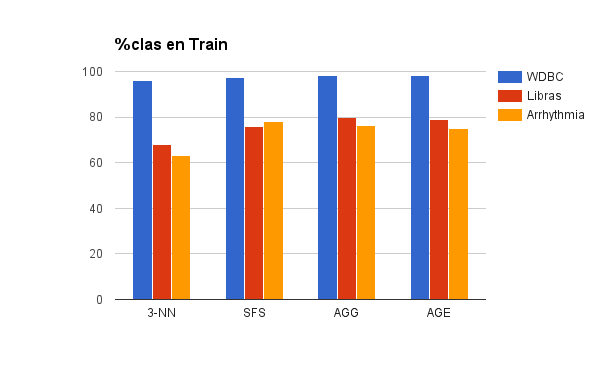
\includegraphics[width=0.7\textwidth]{train}
\caption{Tasa de acierto en el conjunto train} \label{fig:train}
\end{figure}

\begin{figure}[H]
\centering
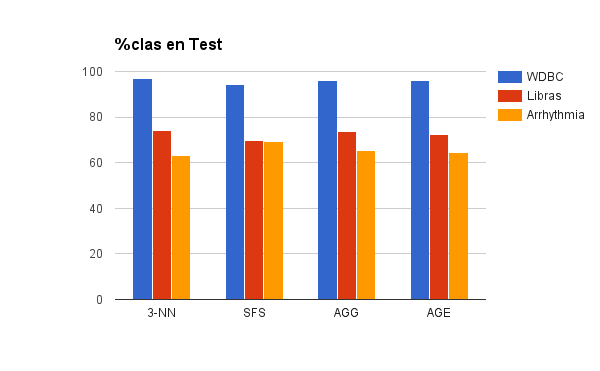
\includegraphics[width=0.7\textwidth]{test}
\caption{Tasa de acierto en el conjunto test} \label{fig:test}
\end{figure}

\begin{figure}[H]
\centering
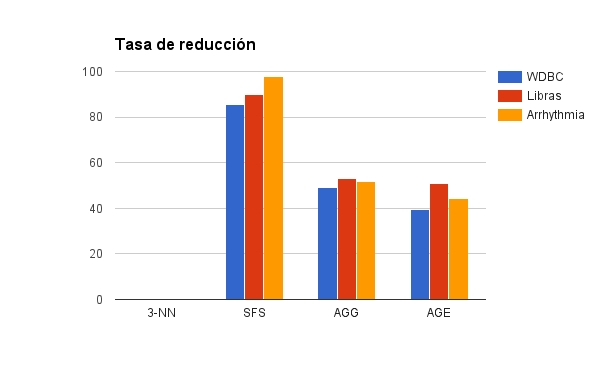
\includegraphics[width=0.7\textwidth]{reduccion}
\caption{Tasa de reducción} \label{fig:reduccion}
\end{figure}

\begin{figure}[H]
\centering
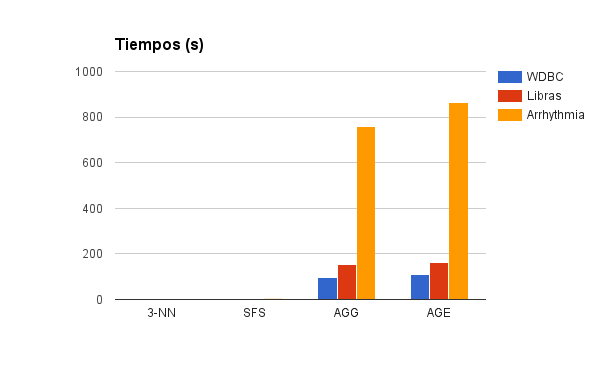
\includegraphics[width=0.7\textwidth]{tiempos}
\caption{Tiempo en segundos} \label{fig:tiempos}
\end{figure}

Vamos a fijarnos primero en las tasas de acierto, tanto de los conjuntos de train como de test. Como podemos ver, en Wdbc había poco margen de mejora (\texttt{SFS} ya obtiene 97,15 en train y 94,48 en test) pero aun así tanto \texttt{AGG} como \texttt{AGE} tienen mejores tasas: cerca de 98,2 en train y cerca de 96 en test los dos. En libras se nota un poco más la mejora, ya que aquí sí se podía mejorar más (\texttt{SFS} tiene 75,8 en train y 69,8 en test) pero sigue siendo poco, ya que en ningún caso hay más de un 5\% de diferencia con \texttt{SFS}. De los dos genéticos, el que tiene más tasa es el generacional, que llega a 79,6 en train y 73,6 en test. Sin embargo en arritmia ninguno de los dos genéticos llega a superar al \texttt{SFS}, quedando el generacional un casi un 2\% por debajo y el estacionario casi un 4\% por debajo en train y casi un 4\% y un 5\% respectivamente por debajo en test. Esto es debido a que en arritmia hay muchas características que no aportan mejora a las soluciones o que incluso empeoran las soluciones, por lo que es lógico el que el \texttt{SFS}, que elige una a una las características que aportan mayor mejora tenga más tasa en bases de datos como esta, ya que en los genéticos no estamos dando prioridad a aquellas soluciones que tienen menor número de características, es decir, no eliminamos de las soluciones características que no aportan nada o que empeoran las soluciones, quizás si se hubiera considerado esto y se hubiera añadido a la implementación, se hubieran obtenido mejores tasas de acierto, sobre todo en arritmia, pero también hubiera aumentado más aún el tiempo que tardar en finalizar el algoritmo, que como vamos a ver ahora, ya es muy alto comparándolo con \texttt{SFS}.\\

Como decíamos, en cuanto a los tiempos, los genéticos tardan más que \texttt{SFS} porque tienen más carga computacional entre la selección, los cruces y las mutaciones, además de que no paran hasta haber llamado 15000 veces a la función de evaluación. Cabe destacar que el generacional, además de obtener mejores tasas, como acabamos de comentar, también tarda un poquito menos que el estacionario (esta diferencia es más significativa en arritmia). Sin embargo en arritmia los dos tardan demasiado para no conseguir ninguna mejora con respecto al \texttt{SFS} por lo que en realidad, si miramos el conjunto, no son buenos para un problema como el de selección de características (estamos hablando de cerca de 14 minutos frente a los segundos que tarda \texttt{SFS} para obtener menor tasa de acierto) en bases de datos grandes con muchas características.\\

Con respecto al 3NN al principio parece raro que tenga menos tasa de acierto que los demás (en la mayoría de los casos) puesto que está considerando todas las características. Sin embargo como hemos comentado, no todas las características tienen que ser buenas definiendo una clase, además de que puede haber ruidos que hayan afectado más a unas que a otras. Es por esto que es normal que tenga un poco menos de acierto y que no haya mucha diferencia entre las tasas de acierto para entrenamiento y para test y además que la de entrenamiento no sea mejor que la de test, puesto que en este algoritmo en realidad las dos serían de test ya que no estamos utilizando ninguno de los dos conjuntos para aprender qué características usar al estar utilizando todas las características.

\section{Bibliografía}
\begin{enumerate}
\item Scipy para leer ficheros arff \href{arff http://docs.scipy.org/doc/scipy/reference/generated/scipy.io.arff.loadarff.html}{aquí}.
\item Documentación de numpy \href{http://docs.scipy.org/doc/numpy/user/index.html}{aquí}.
\item Ficheros para el 3NN \href{https://github.com/agarciamontoro/metaheuristics/tree/master/src/knnGPU}{aquí} (aunque se encuentran también en los ficheros de mi práctica para poder utilizarlos).
\end{enumerate}

\end{document}